\section{Experiments and Comparative Study}\label{sec:experiments}
\researchquestion{RQ1}{Cross-model understanding}{How do general-purpose vision--language models perform on ELEC-VQA?}
\researchquestion{RQ2}{Domain adaptation}{How do answer-only and evidence--answer supervision interact with output prompting?}
\researchquestion{RQ3}{Verifiable evidence}{When does evidence supervision improve supported answers?}
\subsection{Experimental Protocol and Metrics}
The dataset contains 6,972 training, 1,155 validation and 2,074 test QA records. Excluding ten T14 diagnostic controls per evaluation split gives 1,145 validation and 2,064 test questions. The test panel spans seven source DWGs from two projects. Questions and variants sharing a source remain statistically dependent.
The comparators are Qwen2.5-VL-7B-Instruct (Base), its answer-only adapter A, its compact-evidence--answer adapter E, InternVL2\_5-8B and LLaVA-OneVision Qwen2 7B. Adapters use seed 42. Models receive identical questions and raw images with native preprocessing. Greedy decoding allows 768 new tokens. The direct track requests a brief answer without explanation. A second track requests visible components, connections and conditions, followed by a brief final answer, identically for Base/A/E.

Qwen2.5-32B-Instruct is the sole automatic judge. Reference-guided absolute grading follows LAVE~\cite{manas2024lave}; prior Qwen judge evaluations provide precedent~\cite{yu2025risejudge}, not domain-specific validation. Model identities are withheld. Responses receive ratings 3 (full), 2 (task-permitted partial), or 1 (no credit), mapped to semantic scores 1, 0.5 and 0. Binary decisions receive no partial credit. A correct short answer requires no explanation for answer credit. Evidence is scored separately for valid entities, paths, states and support. Joint full credit requires answer and evidence ratings of 3 for the same response. Judge inference uses BF16/SDPA, a 12,288-input-token ceiling, 512 new tokens and one format-recovery retry.

The primary tables include provisional, reference-based supplementary ratings for 585 originally unresolved judgments: 28 direct-answer, 75 explanation-track answer and 482 evidence records. These concern 552 responses to 517 questions, not 585 independent questions. Original non-null Qwen ratings remain fixed. Supplementation combines assistant assessment against the released references with recovery of 85 consistent numerical suggestions from original judge attempts. None has independent human confirmation. These are therefore mixed-evaluator provisional results, not fully automatic or expert-validated scores. The unchanged Qwen-only estimates are retained as a sensitivity analysis. Reference and evaluator errors remain limitations~\cite{zheng2023judge}. No sample is removed to improve a score.

We report QA-micro full-credit accuracy, equal-weight task and drawing macro accuracy, and auxiliary semantic score. T14 is diagnostic and excluded from primary aggregates. A paired bootstrap resamples the seven source DWGs with replacement, retaining all their questions (2,000 replicates, seed 42). Intervals quantify source-resampling variability, not judge bias, supplementary-rating validity or training-seed variability.

\subsection{Cross-Model Answer Results}
A achieves 74.27\% direct-answer full credit, exceeding Base by 37.11 percentage points. E reaches 52.42\%, above Base but below A by 21.85 points. Cross-family baselines remain near 34.5\% (Table~\ref{tab:main}). Native preprocessing and pretraining differences prevent interpreting the comparison as an isolated architectural effect.

\begin{table*}[t]\centering\small
\caption{Direct-answer test results (\%). Supplemented denotes originally unresolved ratings assigned provisional scores; it is not a count of additional test samples.}\label{tab:main}
\begin{tabular}{lrrrrr}\toprule Model & Full credit & Task macro & DWG macro & Semantic & Supplemented\\\midrule
A & 74.27 & 74.98 & 59.89 & 75.34 & 3 \\
E & 52.42 & 52.39 & 40.73 & 52.98 & 3 \\
Base & 37.16 & 33.93 & 42.10 & 38.06 & 11 \\
InternVL2.5-8B & 34.45 & 32.83 & 35.66 & 35.47 & 4 \\
LLaVA-OneVision & 34.54 & 32.28 & 30.47 & 35.00 & 7 \\
\bottomrule\end{tabular}\end{table*}
\subsection{Output Prompt and Evidence Supervision}
Under common explanation prompting, answer accuracy is 39.00\% for Base, 70.16\% for A and 67.97\% for E (Fig.~\ref{fig:effects}). E improves by 15.55 points relative to direct mode, with a drawing-cluster bootstrap interval of [12.63,17.86]. A changes by -4.12 points [-4.92,-2.35]. The explanation-track A-minus-E gap is 2.18 points [-1.61,6.65]. An interval spanning zero establishes neither equivalence nor a stable answer advantage for E. Output alignment and additional generated computation remain alternative explanations; these comparisons do not demonstrate a causal effect of visible reasoning text.

\begin{figure}[t]\centering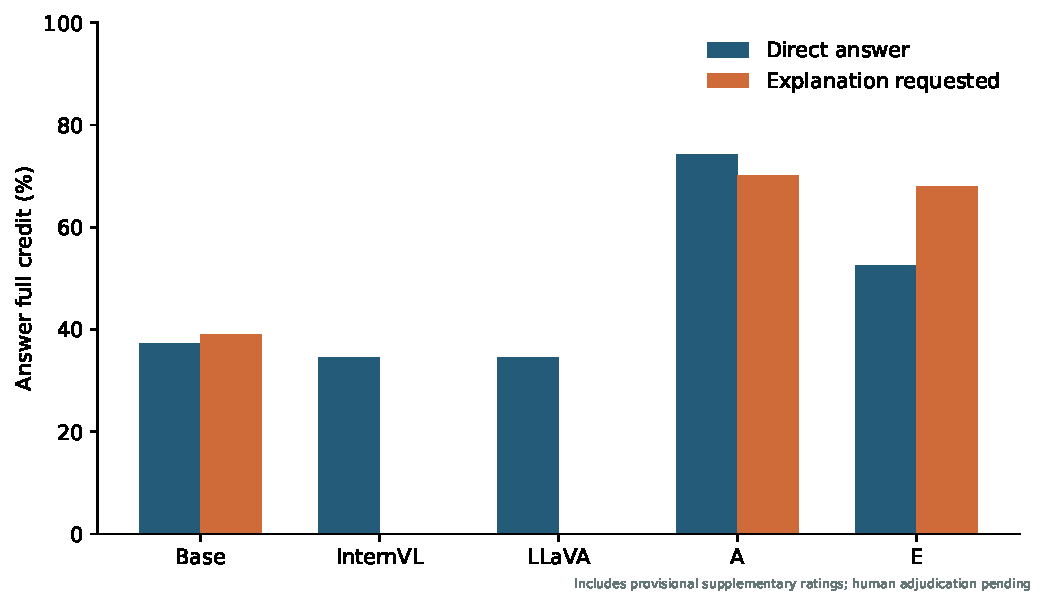
\includegraphics[width=\linewidth]{assets/figure_06.pdf}
\caption{Answer full credit under the two output protocols. Explanation tracks are evaluated for Base/A/E only.}\label{fig:effects}\end{figure}
\subsection{Evidence and Joint Correctness}
E achieves 64.78\% evidence full credit and 64.24\% joint full credit, compared with A's 46.27\% and 46.17\%. The joint improvement is 18.07 points, with a drawing-cluster bootstrap interval [16.04,20.44]. This supports improved reference-supported responses rather than uniformly better final decisions.

\begin{table}[t]\centering\small
\caption{Common explanation-track full credit (\%), including provisional supplementary ratings.}\label{tab:evidence}
\begin{tabular}{lrrr}\toprule Model & Answer & Evidence & Joint\\\midrule
Base & 39.00 & 32.17 & 31.93 \\
A & 70.16 & 46.27 & 46.17 \\
E & 67.97 & 64.78 & 64.24 \\
\bottomrule\end{tabular}\end{table}
A sensitivity analysis with supplementary judgments withheld gives original Qwen-only joint lower estimates are 46.08\% for A and 63.76\% for E; the corresponding unresolved upper bounds are 63.18\% and 64.78\%. Thus, the original E lower estimate exceeds A's original upper bound by 0.58 points within missing-rating assignments. This does not protect against systematic reference or judge error. Original direct-answer estimates are 74.18\% for A and 52.37\% for E, compared with the supplemented values in Table~\ref{tab:main}. The central ordering is preserved.

\begin{figure}[t]\centering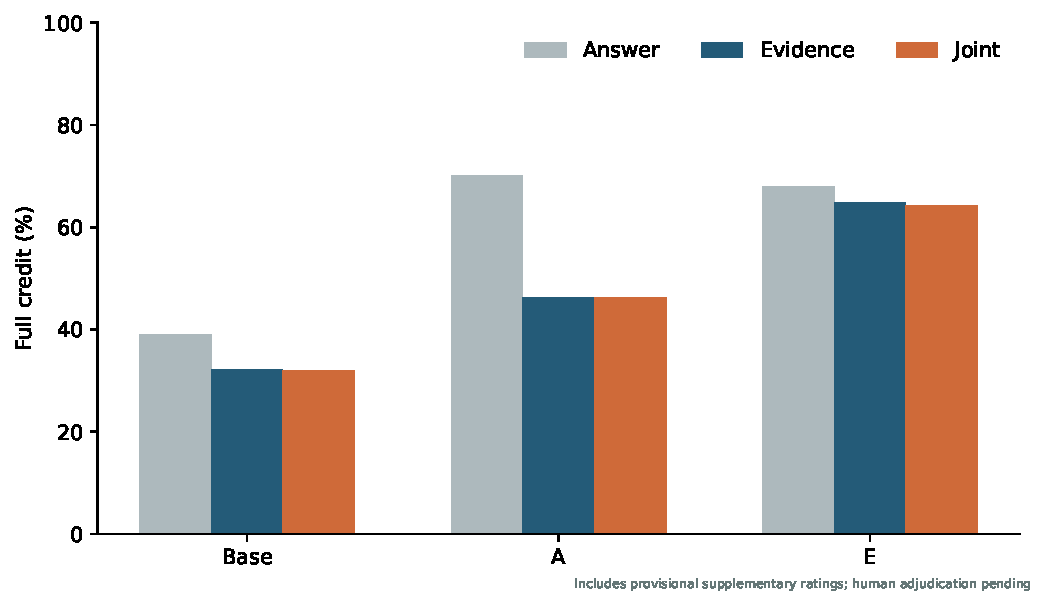
\includegraphics[width=\linewidth]{assets/figure_07.pdf}
\caption{Answer, evidence and joint full credit with common explanation prompting.}\label{fig:evidence}\end{figure}
\subsection{Conditions Under Which E Outperforms A}
E improves answer full credit on measurement planning (T08, +42.52 points), diagnosis sufficiency (T13, +15.00), open-contact impact (T04, +6.63), branch interruption (T15, +7.50) and contact order (T11, +5.26). Conversely, minimum closure, wire grouping and hypothetical bypass remain weaker. Table~\ref{tab:pertask} reports every primary family. Differences are exploratory and are not adjusted for multiple comparisons.
\begin{table}[t]\centering\small
\caption{E minus A under identical explanation prompting (percentage points).}\label{tab:pertask}
\begin{tabular}{lrrr}\toprule Task & N & Answer difference & Joint difference\\\midrule
T01 & 440 & -5.68 & +38.64 \\
T02 & 181 & -9.39 & -13.81 \\
T03 & 200 & -12.50 & -13.50 \\
T04 & 181 & +6.63 & +30.94 \\
T05 & 181 & -5.52 & -4.97 \\
T06 & 181 & -14.36 & -4.97 \\
T07 & 127 & -3.94 & -6.30 \\
T08 & 127 & +42.52 & +44.88 \\
T09 & 200 & -2.00 & +46.50 \\
T10 & 69 & -11.59 & +21.74 \\
T11 & 57 & +5.26 & +7.02 \\
T12 & 40 & -7.50 & +10.00 \\
T13 & 40 & +15.00 & +80.00 \\
T15 & 40 & +7.50 & +50.00 \\
\bottomrule\end{tabular}\end{table}
An original-DWG case asks whether bridging open 2ZJ contact 24--23 connects 3UK:4 to CZ:41 while 3UK contact 3--4 is closed. Both adapters fail under direct prompting; A also fails when explanation is requested. E identifies the visible route 3UK:4 $\rightarrow$ 3UK:3 $\rightarrow$ 2ZJ:24 $\rightarrow$ 2ZJ:23 $\rightarrow$ CZ:41 and answers correctly. This illustrates successful explicit decomposition, not an intervention on internal reasoning.

\begin{figure}[t]\centering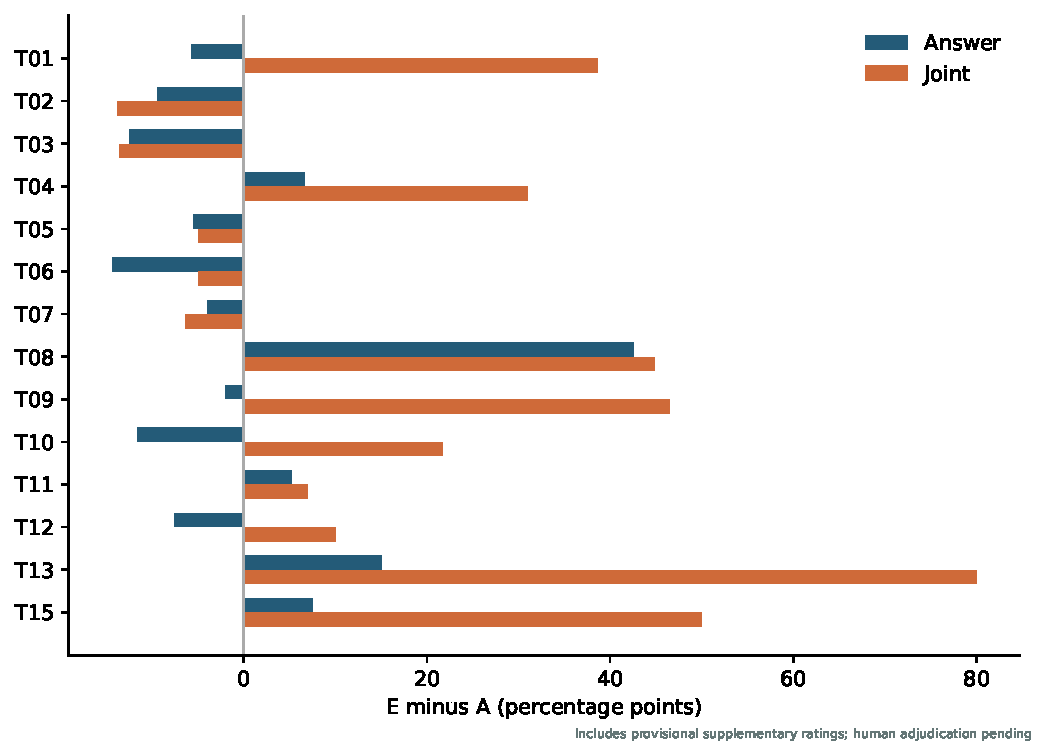
\includegraphics[width=\linewidth]{assets/figure_08.pdf}
\caption{Task-dependent gains and losses for E. All primary families are retained.}\label{fig:taskeffects}\end{figure}
\subsection{Conditional Support and the Answer--Evidence Gap}
Following the distinction between task performance and explanation quality in e-ViL~\cite{kayser2021evil}, let $C_i$ indicate answer full credit and $V_i$ evidence full credit. Conditional support is
\begin{equation}
Q_{E\mid A}=\frac{\sum_i C_iV_i}{\sum_i C_i}.
\end{equation}
The denominator contains correct answers, unlike joint accuracy, which uses the complete question panel. The metric assesses observable support rather than causal faithfulness; sufficiency and comprehensiveness~\cite{deyoung2020eraser} require input interventions and new predictions and are not inferred here.
Conditional support is 65.81\% for A and 94.51\% for E. Accordingly, 34.19\% and 5.49\% of correct answers lack full-credit evidence. This gap indicates that a correct conclusion can coexist with absent, incomplete or incorrect support; those categories should not all be called hallucination. Base attains 81.86\%, but answers fewer questions correctly, so a high conditional value does not imply stronger overall supported reasoning. Conditioning on correct answers also changes the selected subset across models.

\begin{figure}[t]\centering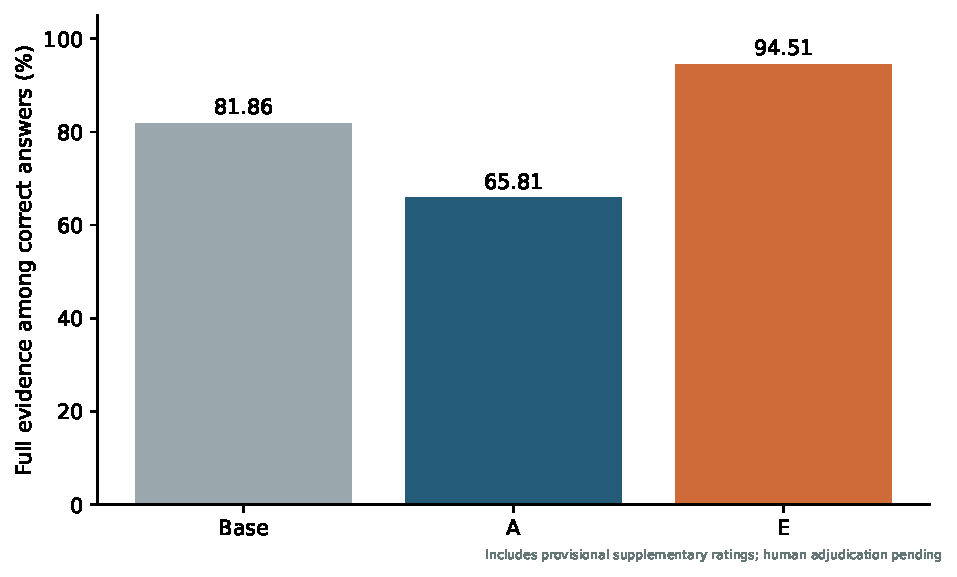
\includegraphics[width=\linewidth]{assets/figure_09.pdf}
\caption{Full-credit evidence conditional on answer full credit, using supplemented ratings.}\label{fig:conditional}\end{figure}
\subsection{Sensitivity to Controlled Changes}
Motivated by consistency analysis in GQA~\cite{hudson2019gqa}, a pair succeeds only when both answers receive full credit; merely changing an output is insufficient. The fixed inventory comprises 69 visual and 179 state pairs. Shared questions and circuits preclude treating them as independent trials.

Under common explanation prompting, E succeeds on 77/82 state-flip pairs (93.90\%) versus A's 55/82 (67.07\%). However, E succeeds on only 11/97 state-invariant pairs (11.34\%) versus A's 60/97 (61.86\%). E improves on visual-invariant pairs (40/46, 86.96\%, versus 36/46, 78.26\%), but is weaker on visual-flip pairs (1/23, 4.35\%, versus 9/23, 39.13\%). Evidence-guided adaptation is therefore more successful for selected relevant state changes but insufficiently selective for irrelevant changes, and weak for topology-changing visual pairs. Better explanation production does not establish robust visual causal understanding.
\begin{figure}[t]\centering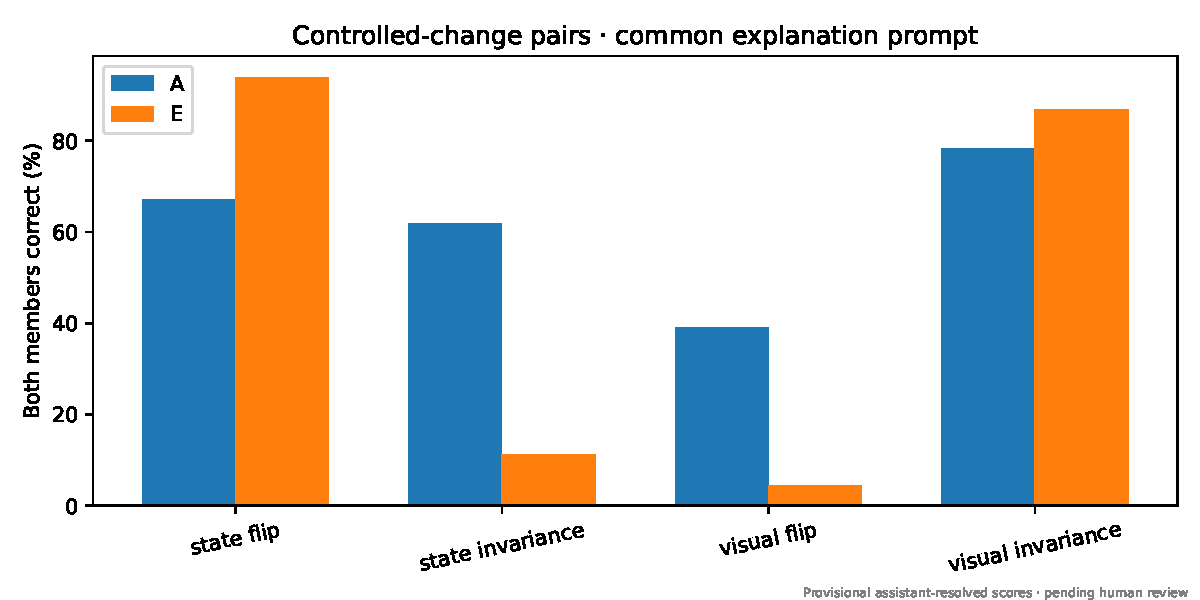
\includegraphics[width=\linewidth]{assets/figure_10.pdf}
\caption{Both-members-correct performance on the fixed change-pair inventory.}\label{fig:pairscores}\end{figure}
\subsection{Reference Complexity and Heterogeneous Gains}
On the 98 questions with at least three explicit reference states, E achieves 63.27\% answer full credit versus 43.88\% for A, a 19.39-point advantage. On the 1,445 two-state questions, they are close (73.08\% versus 73.63\%); E is worse on one-state questions (56.24\% versus 69.58\%). E also exceeds A on recorded paths of four to six edges (61.81\% versus 58.32\%) and seven or more edges (53.00\% versus 49.77\%).

Edge counts concern the bounded reference graph, not visible wire segments or latent reasoning steps. Questions without a recorded path form a separate group. Task composition, answer distribution and complexity are correlated; these exploratory strata do not isolate a causal complexity effect. The findings support improved explicit justification and selective conditional reasoning, alongside topology and relevance failures.
\begin{figure*}[t]\centering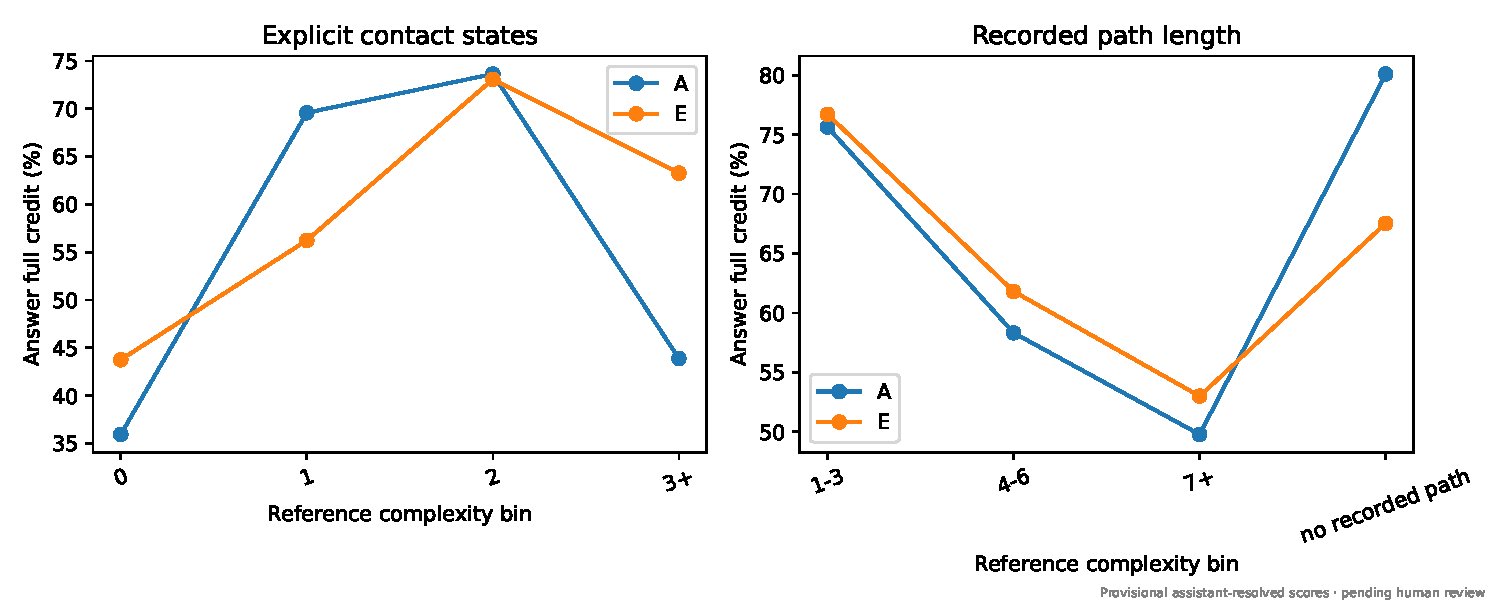
\includegraphics[width=.85\textwidth]{assets/figure_11.pdf}
\caption{Answer full credit by reference-state count and maximum recorded path length. All bins are retained.}\label{fig:complexity}\end{figure*}
\subsection{Generation Cost and Limitations}
Direct-track mean generation times are 0.65, 0.73 and 1.21 seconds for Base, A and E; explanation prompting increases these to 6.67, 0.82 and 2.30 seconds. Mean generated explanation-track lengths are 278.13, 13.10 and 54.81 tokens. A remains brief despite the evidence request. E's evidence advantage incurs additional generation cost. These per-response latencies are not deployment throughput or a hardware-normalized architectural comparison. Efficiency summaries retain all 2,074 test responses, including T14, whereas accuracy aggregates exclude T14.
\begin{figure}[t]\centering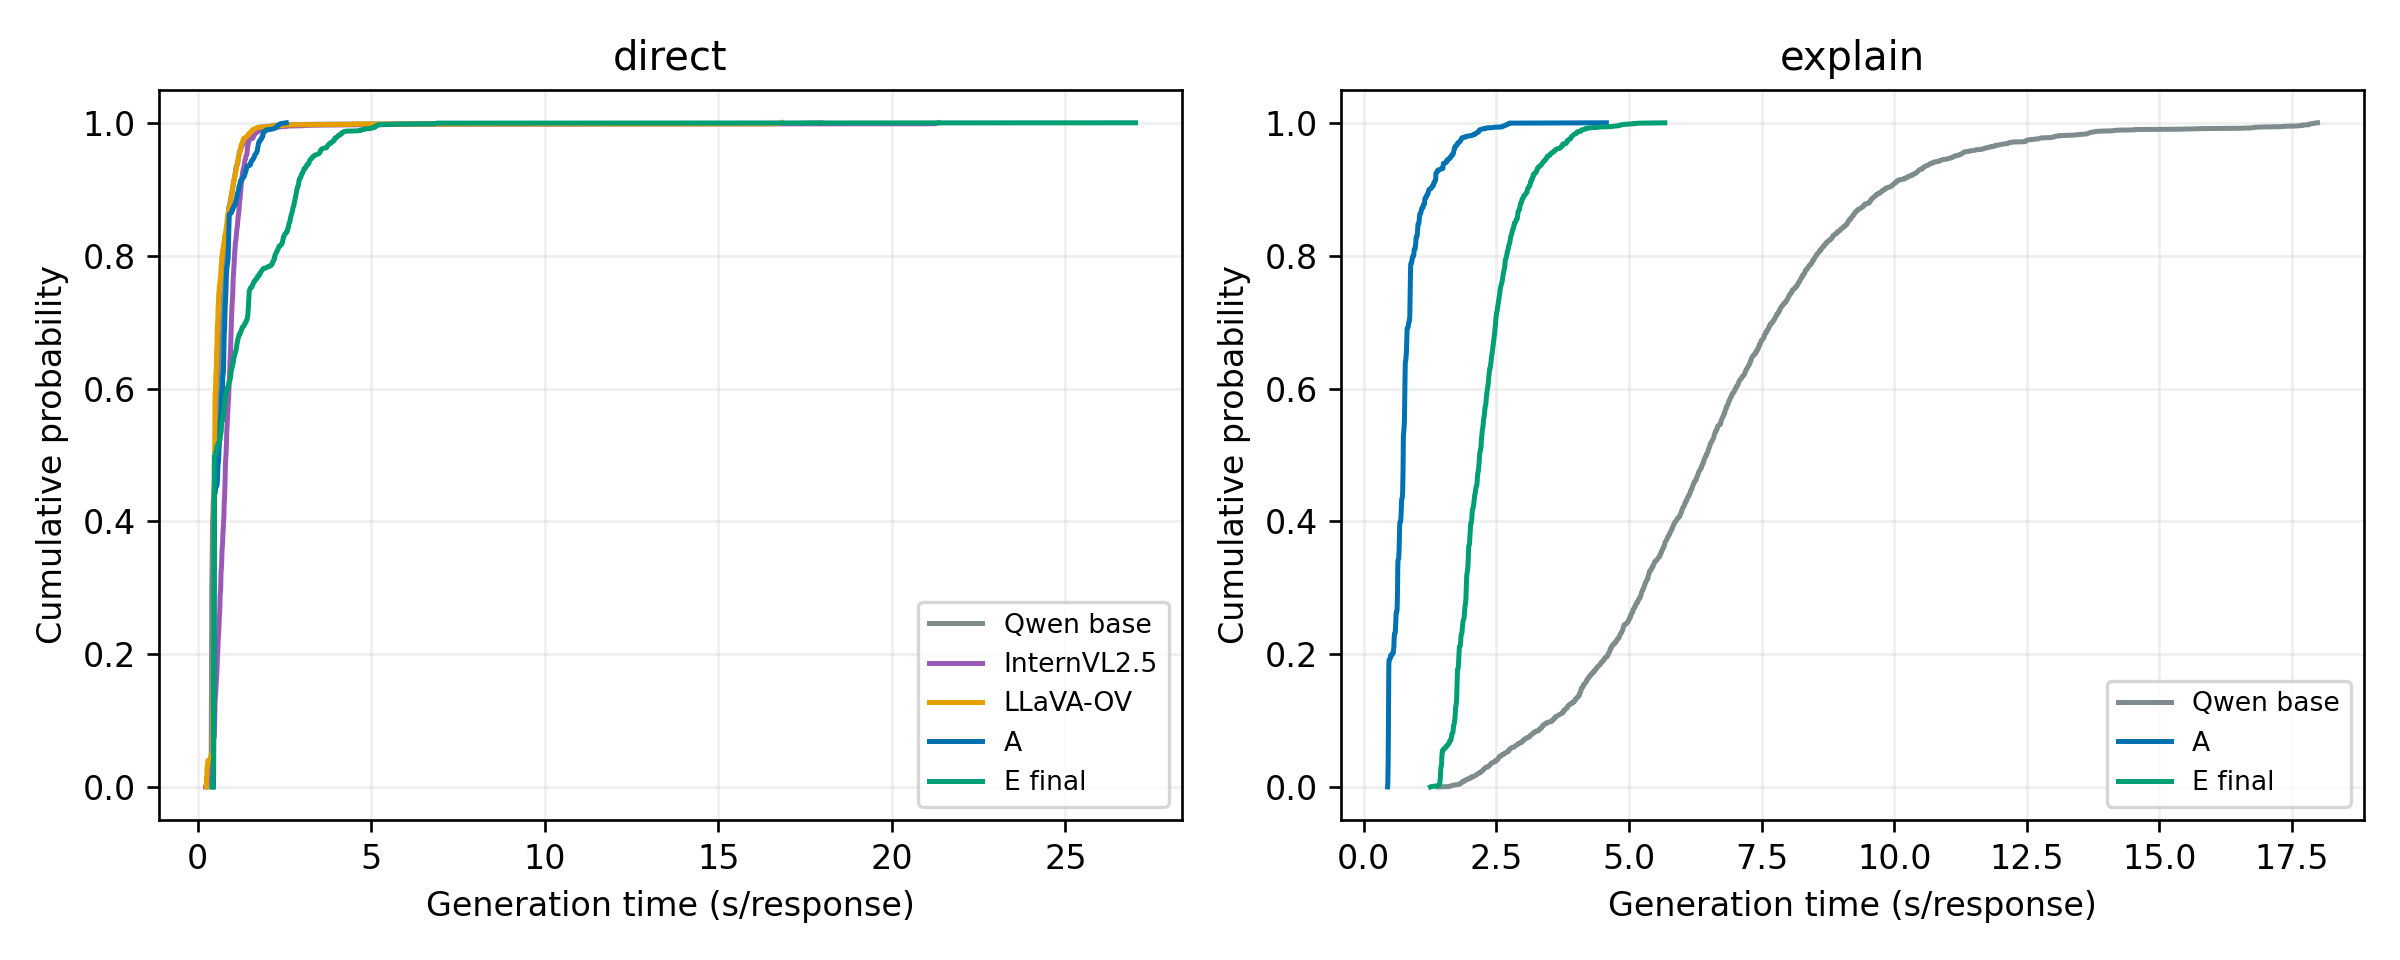
\includegraphics[width=\linewidth]{assets/figure_12.png}
\caption{Generation-latency distributions under the two output protocols.}\label{fig:latency}\end{figure}
The study uses one training seed, seven held-out drawings and references without independent expert validation. Provisional supplementary scoring introduces additional evaluator uncertainty. Domain-adaptation gains and improved supported output are observed within this scope; universal superiority, causal reasoning faithfulness and broad industrial generalization are not established.
